
% COURS 1

\section{Théorie des Graphes}

\subsection{Définitions}

\begin{defn}
Un graphe $\Gamma$ est un triplet $(V,E,\gamma)$ où V est un ensemble fini dont les éléments sont appelés sommets, E est un ensemble fini dont les éléments sont appelés arêtes, $\gamma$ est une fonction $\gamma : E \rightarrow Paires(V)$. On nottera le plus souvent $\Gamma = (V,E)$ en omettant la fonction $\gamma$.\\

Soit $\gamma(e) = \{x,y\}$ pour $e \in E, x,y \in V$:
\begin{center}
	\begin{enumerate}
	\item On dit que x et y sont adjacents.

	\item On dit que e est incidente à x et y. \\
	\end{enumerate}
\end{center}

\end{defn}

\begin{defn}
Soit $\Gamma = (V,E,\gamma)$ un graphe.

\begin{enumerate}
\item $\gamma(e)= \{x,x\}$ pour $e \in E, x \in V$ est appellé un lacet.
\item Si au moins 2 arêtes sont incidentes à 2 mêmes somments, on les appelle arêtes multiples.
\item Un graphe est simple s'il n'a ni lacet, ni arêtes multiples. Dans ce cas, on omet la fonction $\gamma$,on note $\Gamma = (V,E)$ et E est identifié un sous-ensemble de Paires(V). \\
\end{enumerate}
\end{defn}

\begin{defn}
Soit $\Gamma = (V,E)$ un graphe. Le degré d'un sommet $v \in V$ est le nombre d'arêtes incidentes à v, les lacets comptant pour 2 arêtes. On note le degré de v par deg(V).
\end{defn}

\begin{exmp}
Dans la figure suivante, nous avons 2 sommets de degré 4 et 6 sommets de degré 1.
\end{exmp}

\begin{figure}[htb]
	\centering
	\begin{tikzpicture}[>=stealth',shorten >=1pt,auto,node distance=1.5cm,thick,main node/.style={circle,fill=blue!20,draw,font=\sffamily\large\bfseries}]

	\node[main node] (c1) {C};
	\node[main node] (c2) [right of=c1] {C};
	\node[main node] (h1) [above of=c1] {H};
	\node[main node] (h2) [left of=c1] {H};
	\node[main node] (h3) [below of=c1] {H};
	\node[main node] (h4) [above of=c2] {H};
	\node[main node] (h5) [right of=c2] {H};
	\node[main node] (h6) [below of=c2] {H};

	\path[every node/.style={font=\sffamily\small}]
	(c1) edge node [above] {} (h1)
		 edge node [left] {} (h2)
		 edge node [below] {} (h3)
		 edge node [right] {} (c2)
	(c2) edge node [above] {} (h4)
		 edge node [right] {} (h5)
		 edge node [below] {} (h6) ;

	\end{tikzpicture}

	\caption{Exemple degrés des sommets dans la molécule $C_{2}H_{6}$.}
\end{figure}

\begin{thrm}
Soit $\Gamma = (V,E)$, alors $$\sum_{i=1}^{\#V} deg(v_{i}) = 2\#E$$
\end{thrm}

\begin{demo}
Chaque arête contribue 2 fois dans la somme des degrés.
\end{demo}

\begin{corll}
La somme des degrés des sommets d'un graphe est paire. \\
\end{corll}

\begin{defn}
Le graphe complet $K_{n}$ est le graphe simple à n sommets pour lequel chaque paire de sommets est une arête.
\end{defn}

\begin{exmp}
	\begin{minipage}{.2\textwidth}
	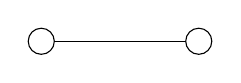
\begin{tikzpicture}
	 \def \radius {1cm}
	 \def \margin {8}
	 \def \n {2}
	 \foreach \s in {1,...,\n}
	  \node[draw, circle] (\s) at ({360/\n * (\s - 1)}:\radius) {};
	 \foreach \s in {1,...,\n}
	  \foreach \t in {\s,...,\n}
	   \draw (\t) -- (\s);
	\end{tikzpicture}
\end{minipage}
\begin{minipage}{.2\textwidth}
	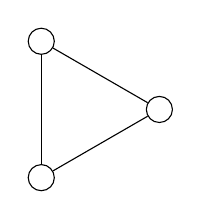
\begin{tikzpicture}
	 \def \radius {1cm}
	 \def \margin {8}
	 \def \n {3}
	 \foreach \s in {1,...,\n}
	  \node[draw, circle] (\s) at ({360/\n * (\s - 1)}:\radius) {};
	 \foreach \s in {1,...,\n}
	  \foreach \t in {\s,...,\n}
	   \draw (\t) -- (\s);
	\end{tikzpicture}
\end{minipage}
\begin{minipage}{.2\textwidth}
	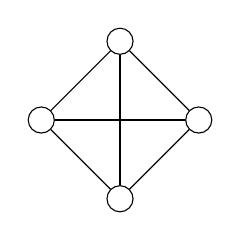
\begin{tikzpicture}
	 \def \radius {1cm}
	 \def \margin {8}
	 \def \n {4}
	 \foreach \s in {1,...,\n}
	  \node[draw, circle] (\s) at ({360/\n * (\s - 1)}:\radius) {};
	 \foreach \s in {1,...,\n}
	  \foreach \t in {\s,...,\n}
	   \draw (\t) -- (\s);
	\end{tikzpicture}
\end{minipage}
\begin{minipage}{.2\textwidth}
	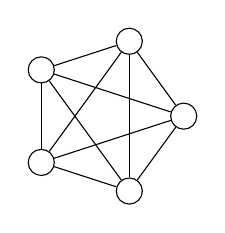
\begin{tikzpicture}
	 \def \radius {1cm}
	 \def \margin {8}
	 \def \n {5}
	 \foreach \s in {1,...,\n}
	  \node[draw, circle] (\s) at ({360/\n * (\s - 1)}:\radius) {};
	 \foreach \s in {1,...,\n}
	  \foreach \t in {\s,...,\n}
	   \draw (\t) -- (\s);
	\end{tikzpicture}
\end{minipage}
\begin{minipage}{.2\textwidth}
	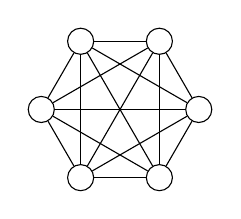
\begin{tikzpicture}
	 \def \radius {1cm}
	 \def \margin {8}
	 \def \n {6}
	 \foreach \s in {1,...,\n}
	  \node[draw, circle] (\s) at ({360/\n * (\s - 1)}:\radius) {};
	 \foreach \s in {1,...,\n}
	  \foreach \t in {\s,...,\n}
	   \draw (\t) -- (\s);
	\end{tikzpicture}
\end{minipage}
\end{exmp}

\begin{defn}
Un graphe ${\Gamma}'=(U,F)$ est un sous-graphe de $\Gamma=(V,E)$ si $ U \subseteq V$ et $F \subseteq E$. On nottera $ {\Gamma}' \leq \Gamma$.
\end{defn}

\begin{exmp}
$ K_{m} \leq K_{n}$ si $ m \leq n$.
\end{exmp}

\begin{exo}
Montrer que $K_{m}$ possède $ q=\frac{1}{2}n(n-1)$ arêtes.
\end{exo}

%----------------------------------------------------

\subsection{Chemins dans les graphes}

\begin{defn}
Soit $\Gamma = (V,E)$ et $v,w \in V$. Un chemin de v à w de longueur n est une séquence alternée de $(n+1)$ sommets $v_{0},v_{1},...,v_{n}$ et de n arêtes $e_{1},e_{2},...,e_{n}$ de la forme $$ (v_{0},e_{1},v_{1},e_{2},...,e_{n},v_{n})$$ dans laquelle chaque $e_{i}$ est incident à $v_{i-1}$ et $v_{i}$ pour $1 \leq i \leq n$ et $ e_{i} \neq e_{j} , \forall i \neq j \in 1,...,n$ \\

Un chemin est simple si aucun sommet ne se répète sauf peut-être $v_{0}$ et $v_{n}$. \\

Dans un graphe simple on nottera juste la suite des sommets lorsque l'on décrit un chemin. \\

\end{defn}

\begin{defn}
Un graphe $\Gamma = (V,E)$ est connexe si $\forall x,y \in V : \exists $ un chemin de x à y. \\

La composante connexe de $\Gamma$ contenant x est le sous-graphe ${\Gamma}'$ de $\Gamma$ dont les sommets et les arêtes sont contenus dans un chemin de $\Gamma$ démarrant en x. \\
\end{defn}

\begin{defn}
Soit $\Gamma = (V,E)$ et $v \in V$.\\

Un cycle est un chemin de v à v.\\

Un cycle simple est un cycle de v à v dans lequel aucun sommet n'est répété (mis à part le départ et l'arrivée).\\
\end{defn}

%----------------------------------------------------

\subsection{Arbres}

\begin{defn}
Un arbre est un graphe simple connexe qui ne contient aucun cycle.\\
\end{defn}

\begin{defn}
Dans un arbre, les sommets de degré 1 sont appellés les feuilles.\\
\end{defn}

\begin{exmp}
<Dessin Arbre>
\end{exmp}

\begin{prop}
Si T est un arbre avec $p\geq2$ sommets, alors T contient au moins 2 feuilles.
\end{prop}

\begin{demo}
T a p sommets. Tous les chemins sont de longueur inférieure ou égale à p. Considérons un chemin $v_{0},v_{1},...,v_{r}$ pour $v_{i} \in V$, $i=0,...,r$ de longueur maximale. Alors, $v_{0}$ et $v_{r}$ sont de degré 1.\\
\end{demo}

\begin{thrm}
Soit T un graphe simple à p sommets. Alors les 3 assertions suivantes sont équivalentes:
	\begin{enumerate}
	\item T est un arbre.
	\item T a $(p-1)$ arêtes et aucun cycle.
	\item T a $(p-1)$ arêtes et est connexe.
	\end{enumerate}
\end{thrm}

\begin{demo}
<Démonstration en 2 parties>.
\end{demo}

% COURS 2

\newpage
<-- COURS 2 MISSING -->
\newpage

% COURS 3

\begin{thrm}[Dirac 1950]
Soit $\Gamma = (V,E)$ un graphe simple avec $p \geq 3$ sommets. Si $\forall v \in V: deg(v) \geq \frac{1}{2}p$, alors $\Gamma$ est Hamiltonien.
\end{thrm}

\begin{demo}
$\Gamma$ est connexe. Soit C = $(v_{0},v_{1},...,v_{k})$ un plus long chemin simple dans $\Gamma$ avec $v_{0} \neq v_{k}, k < p$.\\

$ deg(v_{0}) \geq \frac{p}{2}$, tous les sommets adjacents à $v_{0}$ sont dans $\{v_{1},...,v_{k}\}$\\

$ deg(v_{k}) \geq \frac{p}{2}$, tous les sommets adjacents à $v_{k}$ sont dans $\{v_{0},...,v_{k-1}\}$\\

Comme $k < q$, il doit exister $i \in \{0,...,k-1\}$ tel que $\{v_{i},v_{k}\} \in E$ et $\{v_{0},v_{i+1}\} \in E$. On obtient un cycle $\widetilde{C} = (v_{0},v_{1},...,v_{i},v_{k},v_{k-1},...,v_{i+1},v_{0})$ \\

\begin{figure}[htb]
	\centering
	\begin{tikzpicture}[mydot/.style={fill,circle,inner sep=2pt},]

		\node[mydot,label={$v_{0}$}] (v0) {};
		\node[mydot,below right=of v0] (v1) {};
		\node[mydot,above right=of v1] (v2) {};
		\node[mydot,below right=of v2,label={$v_{i}$}] (v3) {};
		\node[mydot,above right=of v3,label={$v_{i+1}$}] (v4) {};
		\node[mydot,below right=of v4] (v5) {};
		\node[mydot,above right=of v5] (v6) {};
		\node[mydot,right=of v6] (v7) {};
		\node[mydot,above right=of v7] (v8) {};
		\node[mydot,above right=of v8,label={$v_{k}$}] (v9) {};
		\begin{pgfonlayer}{background}
		\Twocolor{(v0)}{(v1)}{red}{green}
		\Twocolor{(v1)}{(v2)}{red}{green}
		\Twocolor{(v2)}{(v3)}{red}{green}
		\Twocolor{(v4)}{(v5)}{green}{red}
		\Twocolor{(v5)}{(v6)}{green}{red}
		\Twocolor{(v6)}{(v7)}{green}{red}
		\Twocolor{(v7)}{(v8)}{green}{red}
		\Twocolor{(v8)}{(v9)}{green}{red}
		\end{pgfonlayer}
		\draw[red,line width=1pt] 
			(v3) -- (v4);
		\draw[green,line width=1pt] 
			(v0) to[out=45,in=135] (v4)
			(v3) to[out=-45,in=-20,looseness=1] (v9);
	\end{tikzpicture}

	\caption{Les 2 chemins, C en rouge, $\widetilde{C}$ en vert.}
\end{figure}

On nq(?) $\widetilde{C}$ est un cycle Hamiltonien.\\

Supposons:\\

$\exists  y \in \widetilde{C} \Rightarrow$ On peut supposer que $\{ v_{j},y\} \in E$ pour $j=\{0,...,k\}$.\\

$\Rightarrow$ On construit un chemin $\overline{C} = (y, v_{j},v_{j-1},...v_{0},v_{i+1},...,v_{k},v_{i},v_{i-1},...,v_{j-1})$. $\overline{C}$ est un chemin plus long que C.

<Second Dessin>

\end{demo}

Illustration: Code de Gray

Un code de Gray d'ordre n est un arrangement cyclique de $2^{n}$ mots binaires de longueur n tels que 2 mots adjacents ne diffèrent qu'en une seule position.\\

\begin{exmp}
<dessin cercles concentriques>
\end{exmp}

Le code de Grey ci-dessus provient d'un cycles Hamiltonien.\\

<dessin cube et cycle>\\

Un code de Gray d'ordre (n+1) se construit à partir d'un code de Gray d'ordre n comme suit:

\begin{enumerate}
\item On écrit le code de Gray donné d'ordre n en ajoutant à la fin de chaque mot un zero.
\item On le fait suivre par le même code de Gray parcouru dans l'autre sens et en ajoutant à la fin de chaque mot un 1.
\end{enumerate}

%----------------------------------------------------

\subsection{Graphes Eulériens}

\begin{defn}
Un cycle Eulérien dans un graphe $\Gamma$ est un cycle qui contient toutes les arêtes de $\Gamma$.
Un graphe est Eulérien s'il contient un cycle Eulérien.\\
\end{defn}

\begin{exmp}
SOME EXAMPLE\\
\end{exmp}

\begin{prop}
Si un graphe est Eulérien, alors tous ses sommets sont de degré pair.\\
\end{prop}

\begin{lemme}
Soit $\Gamma$ un graphe dans lequel chaque sommet est de degré pair, alors l'ensemble E se partitionne en une union de cycles (arête-)disjointe.\\
\end{lemme}

\begin{exmp}
<DRAWING 3 CYCLES>\\
\end{exmp}

\begin{demo}
Par récurrence, sur le nombre d'arêtes
	\begin{enumerate}
		\item Le lemme est vrai pour $q=2$.
		\item Supposons qu'il soit vrai pour tout graphe à $q \leq k$ arêtes et montrons-le pour un graphe à (k+1) arêtes.
		\item Soit $v_{0}$ un sommet de $\Gamma$. On démarre un chemin en $v_{0}$ et on le suit jusqu'à ce qu'un sommet soit répété 2 fois. On le note $v_{j}$ et C le cycle de $v_{j}$ à $v_{j}$.
		\item Soit ${\Gamma}'$ le sous-graphe de $\Gamma$, obtenu par $V={V}'$ et ${E}'=E \setminus C$. ${\Gamma}'$ a $\#{E}' \leq k$ arêtes. Par hypothèse de récurence, les arêtes de ${\Gamma}'$ se partitionnent en une union arête-disjointe de cycles $C_{1} \cup C_{2} \cup ... \cup C_{n}$.
		\item Donc, $C_{1} \cup C_{2} \cup ... \cup C_{n}$ est une partition arête-disjointe des arêtes de $\Gamma$.
		\item RECHECK THIS DEMO, SEEMS FISHY\\
	\end{enumerate}
\end{demo}

\begin{thrm}
Soit $\Gamma$ un graphe connexe. Alors, $\Gamma$ est eulerien si et seulement si chaque sommet a un degré pair.\\
\end{thrm}

\begin{demo}
$\Rightarrow$ OK par proposition précédente.\\
$\Leftarrow$ Par le Lemme: E se partitionne en une union (arête-)disjointe de cycles $C_{1} \cup C_{2} \cup ... \cup C_{n}$.
	\begin{enumerate}
		\item Si n=1, c'est bon.
		\item Si $n>1$, comme $\Gamma$ est connexe, $\exists$ une arête incidente à un $v \in C_{1}$ et un $w \notin C_{1}$. Cette arête est dans $C_{j}$ pour un $j=2,...,n$ (car on a une partitien de E). On attache ce cycle en v. S'il reste des cycles dans la partition, on itère ce procédé jusqu'à avoir utilisé tous les cycles.\\
	\end{enumerate}
\end{demo}
%----------------------------------------------------

\subsection{Application: le problème du voyageur de commerce (TSP)}

\subsubsection{Énoncé du problème}

Énoncé: Un vendeur de livres démarre de chez lui et doit visiter un certain nombre de librairies avant de rentrer chez lui. Comment doit-il choisir sa route pour minimiser la distance parcourue? \\ 

Objet mathématique: Un graphe valué (à chaque arête est associé un nombre appelé poids) où les sommets représentent les librairies et les arêtes représentent les routes.\\

<VALUED K5 GRAPH HERE>\\

Objectif: Trouver un cycle hamiltonien de poids minimal.\\

Remarque: Un graphe complet $K_{n}$ à n sommets possède $\frac{1}{2}(n-1)!$ cycles hamiltoniens differents. Par exemple, pour $n=10 \Rightarrow$ 181440 cycles. On ne connait pas encore d'algorithme efficance qui donne une solution au problème.\\

\subsubsection{Arbres couvrant minimum}

\begin{defn}
Un arbre couvrant dans un graphe $\Gamma$ est un arbre qui est un sous-graphe de $\Gamma$ et qui contient tous les sommets de $\Gamma$.\\
\end{defn}

\begin{exmp}
<GRAPH TO MIN SPANNING TREE EXAMPLES HERE>\\
\end{exmp}

Il existe un algorithme qui donne des arbres couvrants de poids minimum dans un graphe valué.\\

Algorithme de Kurskal:
\begin{enumerate}[i]
\item Choisir une arêtes de plus petit poids.
\item Choisir parmi les arêtes restantes une arête de plus petit poids dont l'inclusion ne crée pas un cycle.
\item Continuer jusqu'à obtenir un arbre couvrant.\\
\end{enumerate}

\begin{exmp}
<GRAPH K5 WITH PATH HERE>\\
\end{exmp}

Remarque: Si C est un cycles hamiltonien dans un graphe $\Gamma$, alors $\forall e \in E$ arête de C: $ C \setminus\{e\}$ est un arbre couvrant.\\

$\Rightarrow$ (Solution de TSP) $\geq$ (longueur minimum d'un arbre couvrant)\\

Mieux: Soit v un sommet de $\Gamma$. Tout cycle hamiltonien contient 2 arêtes incudentes à v. Le reste du chemin est un arbre couvrant de $\Gamma \setminus\{v\}$.\\

$\Rightarrow$ (Solution de TSP) $\geq (\sum$ des longueurs des 2 plus courtes arêtes incidentes à v) + (longueur minimum d'un arbre couvrant de $\Gamma \setminus\{v\}$)\\

Remarque: $\exists$ borne supérieure à TSP en utilisant des cycles euleriens. \\

\subsection{Ordres partiels}

\begin{defn}
Soit P un ensemble. Un ordre partiel sur P est une relation sur P, c'est à dire un ensemble de couples $(p_{1},p_{2}) \in P\times P$, noté $p{1} \leq p{2}$ tel que:
	\begin{enumerate}
		\item $p \leq p$ (réflexive)
		\item $(p \leq q$ et $q \leq p ) \Rightarrow p = q$ (anti-symétrique)
		\item $(p \leq q$ et $q \leq r ) \Rightarrow p \leq r$ (transitive)\\
	\end{enumerate}
On note $(P,\leq)$ un ensemble partiellement ordonné.\\
\end{defn}

\begin{exmp}
	\begin{enumerate}
		\item $(\mathbb{N},\leq)$
		\item $(\mathbb{N},\mid)$ où $a \mid b$ si $\exists c \in \mathbb{Z}$ tel que $a \cdot c = b$ $(a,b \in \mathbb{Z})$\\
	\end{enumerate}
\end{exmp}


% COURS 4

\newpage
<-- COURS 4 MISSING -->
\newpage


% COURS 3
